\documentclass{amsart}


\usepackage{graphicx}
\usepackage{geometry}
\geometry{
	top=2.5cm,
	bottom=2.5cm,
	left=2cm,
	right=2cm
}

\title{Advanced Macroeconomics III - Replication of Cochrane and Piazzesi (2008)}
\author{Rubén Fernández-Fuertes}

%\newcommand{\includefigure}[1]{
%
%	\
%}

\begin{document}
	\maketitle


	\begin{table}[h!]
		\centering
		\input{tab/table1.txt}
	\end{table}


	\begin{table}[h!]
		\centering
		\input{tab/table2.txt}
	\end{table}


	\begin{figure}[h!]
		\centering
		\includegraphics[scale=0.5]{fig/eps/Figure3.eps}
	\end{figure}

	\begin{figure}[h!]
		\centering
		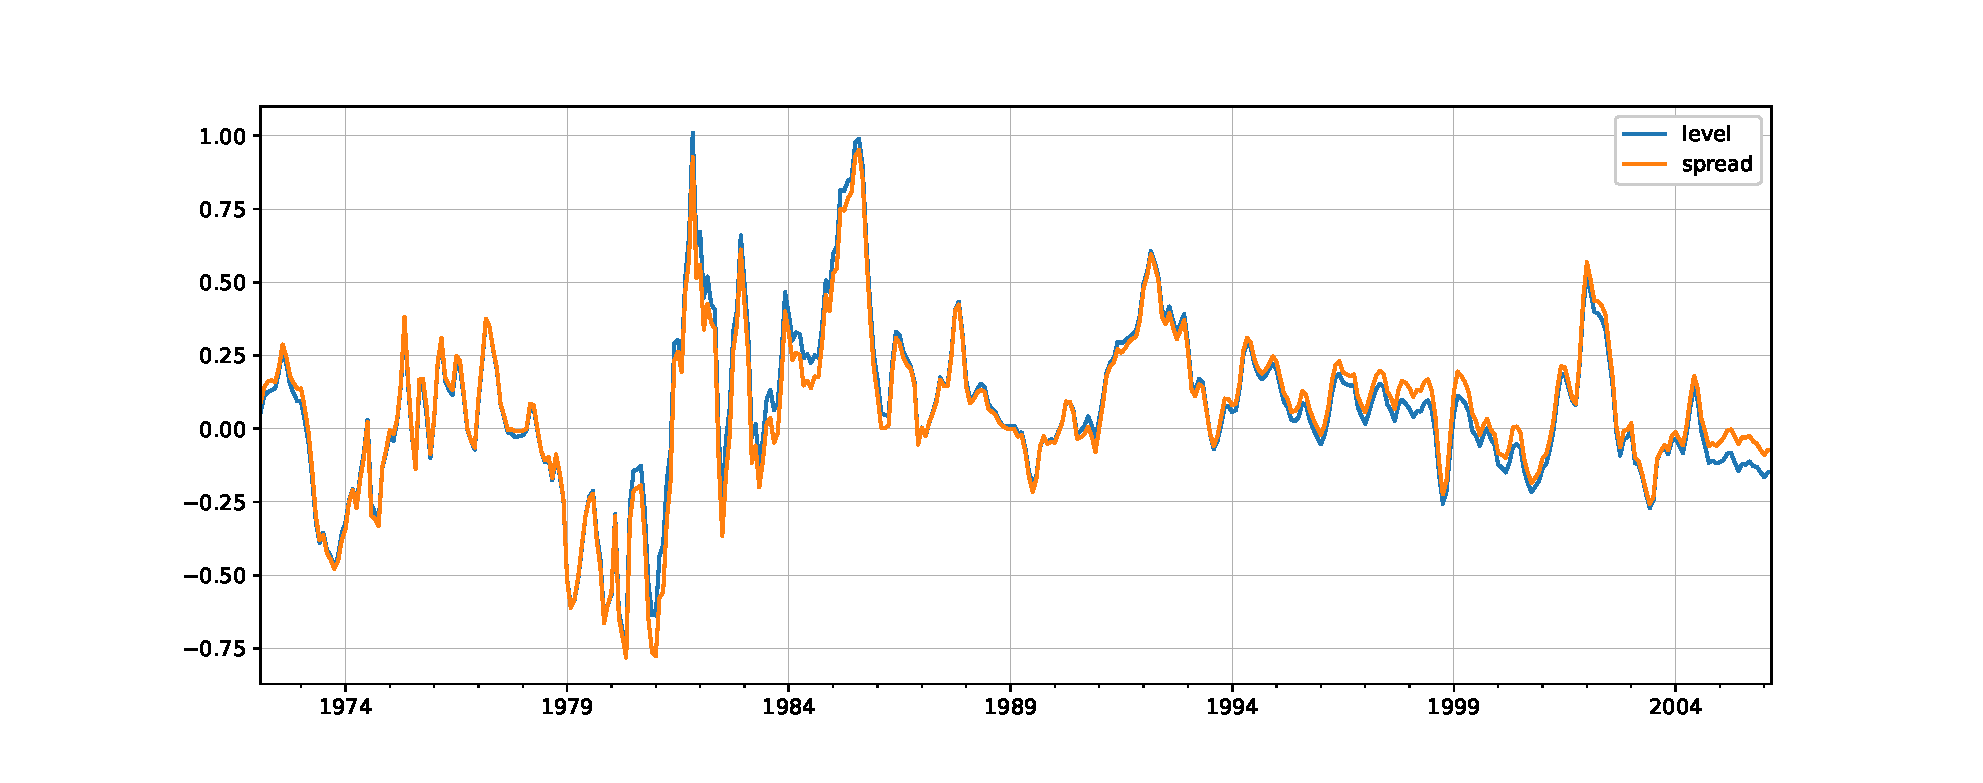
\includegraphics[scale=0.5]{fig/eps/Figure4.eps}
	\end{figure}

	\begin{figure}[h!]
		\centering
		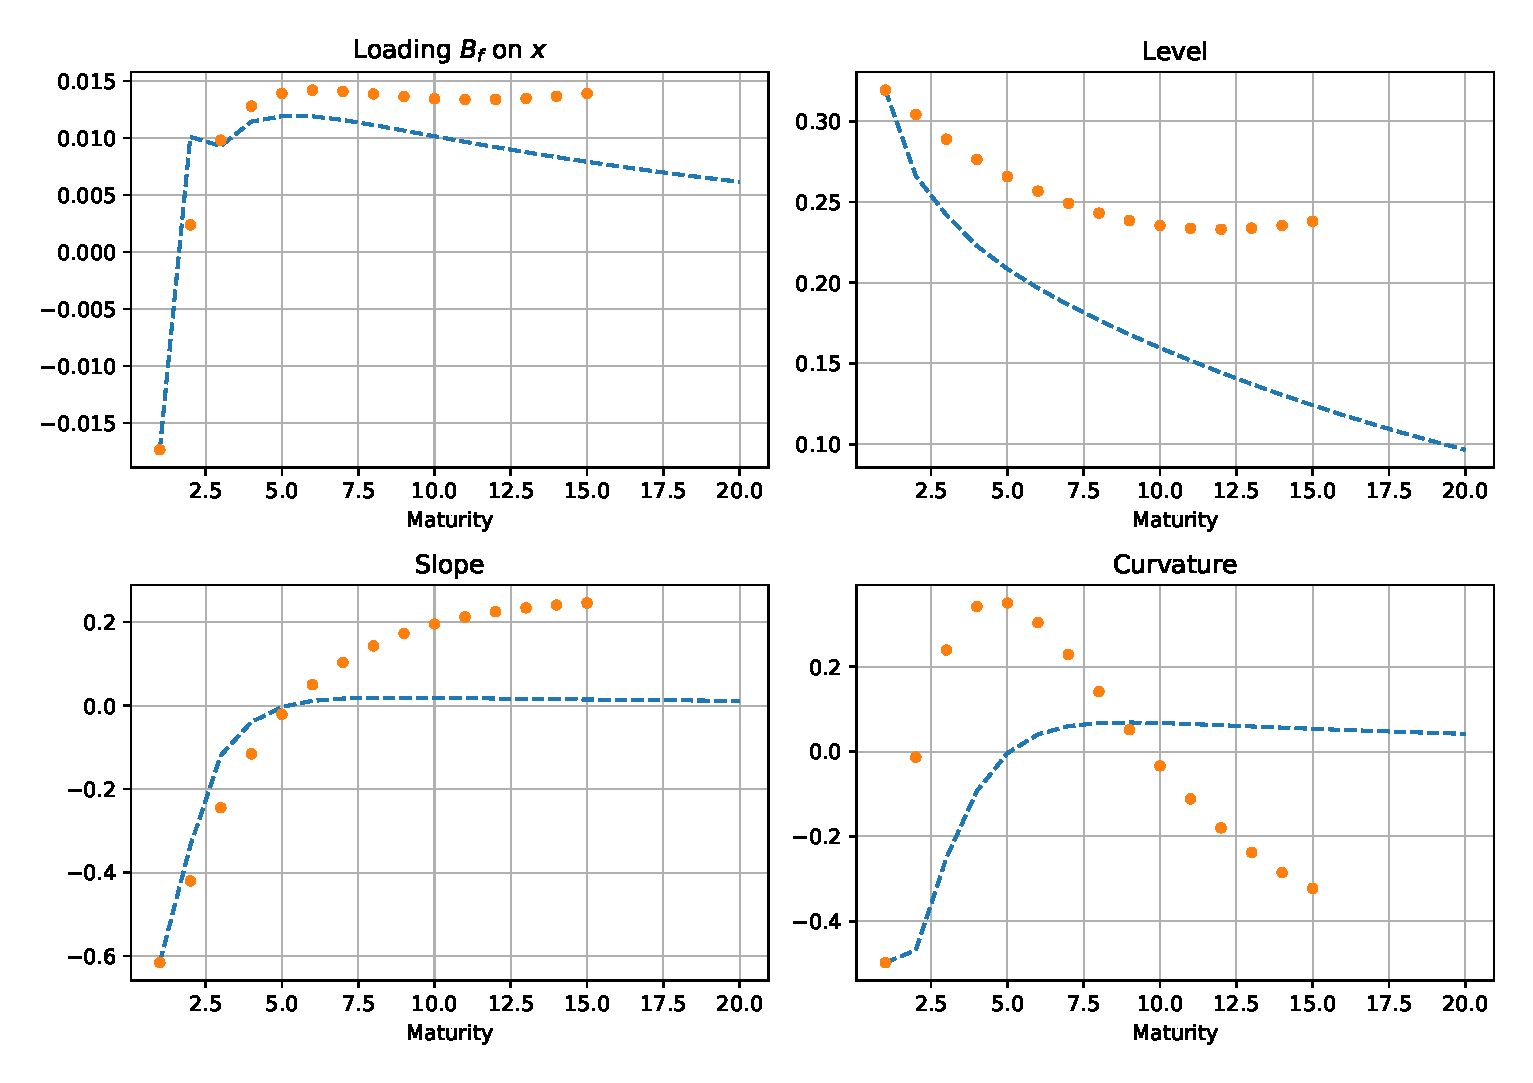
\includegraphics[scale=0.5]{fig/eps/Figure5.eps}
	\end{figure}

	\begin{figure}[h!]
		\centering
		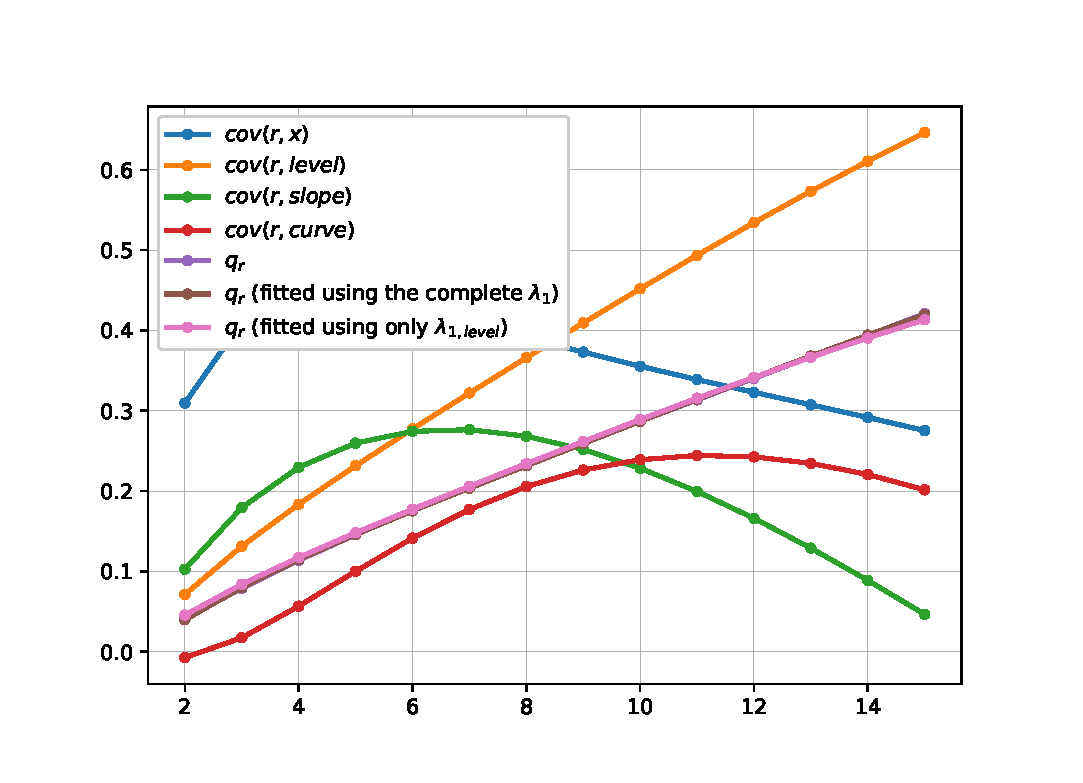
\includegraphics[scale=0.5]{fig/eps/Figure6.eps}
	\end{figure}

	\begin{figure}[h!]
		\centering
		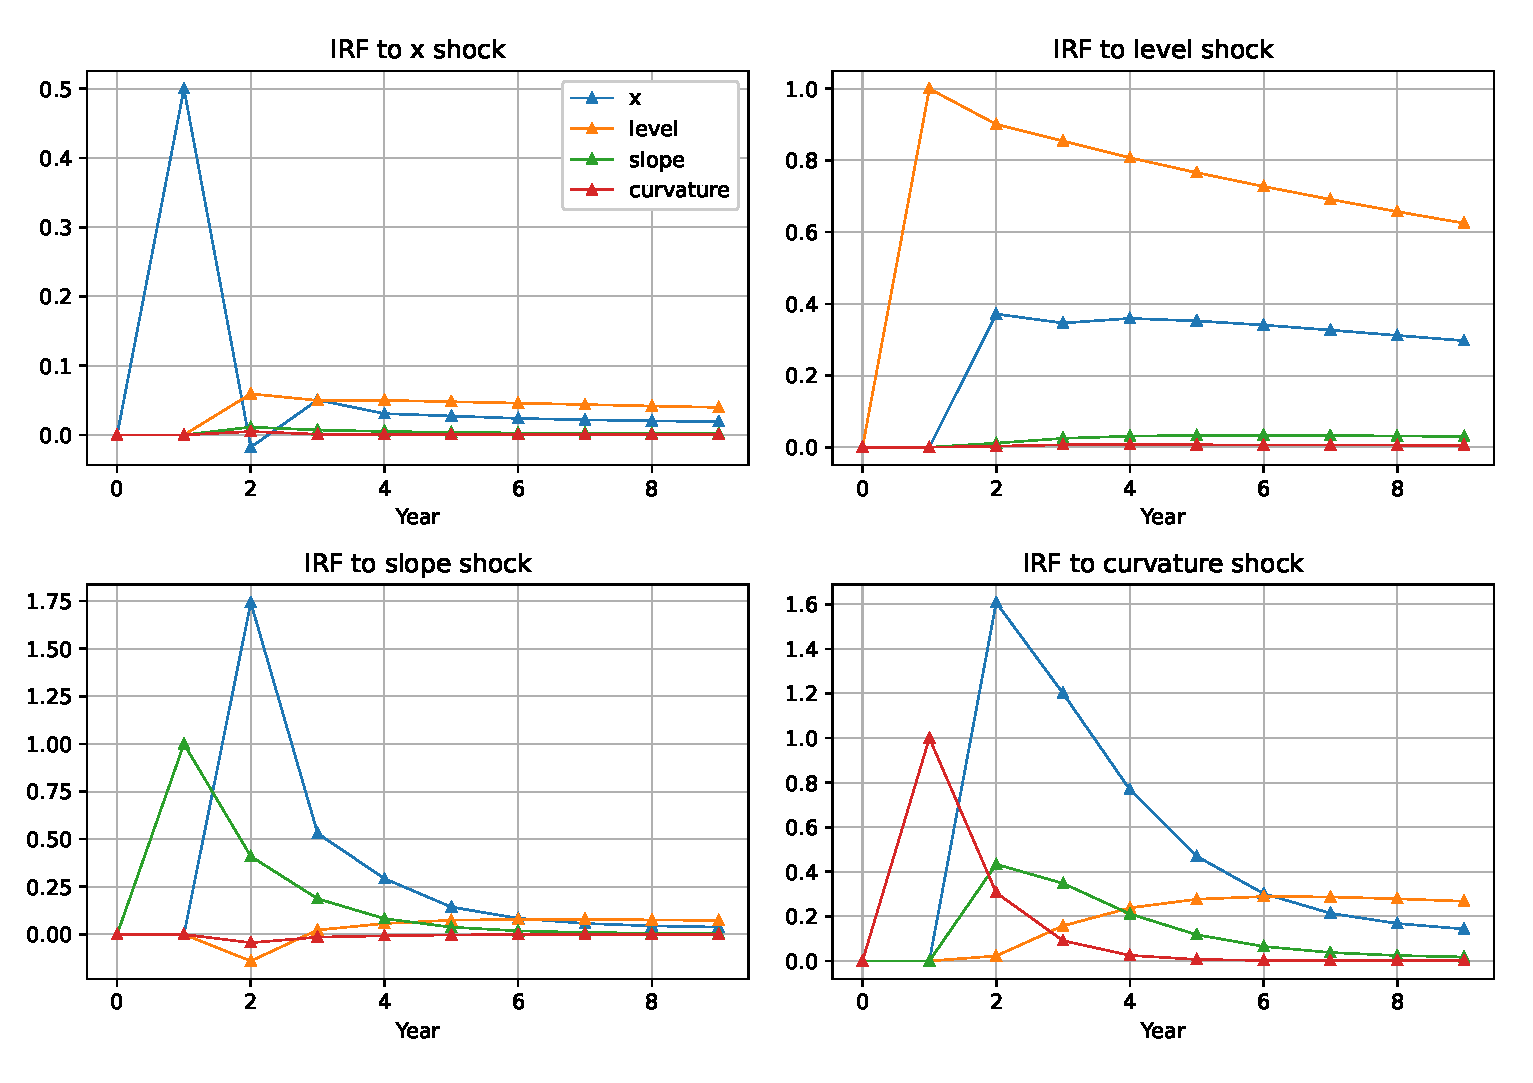
\includegraphics[scale=0.5]{fig/eps/Figure7.eps}
	\end{figure}

	\begin{figure}[h!]
		\centering
		\includegraphics[scale=0.5]{fig/eps/Figure8.eps}
	\end{figure}

	\begin{figure}[h!]
		\centering
		\includegraphics[scale=0.5]{fig/eps/Figure9.eps}
	\end{figure}


	\begin{figure}[h!]
		\centering
		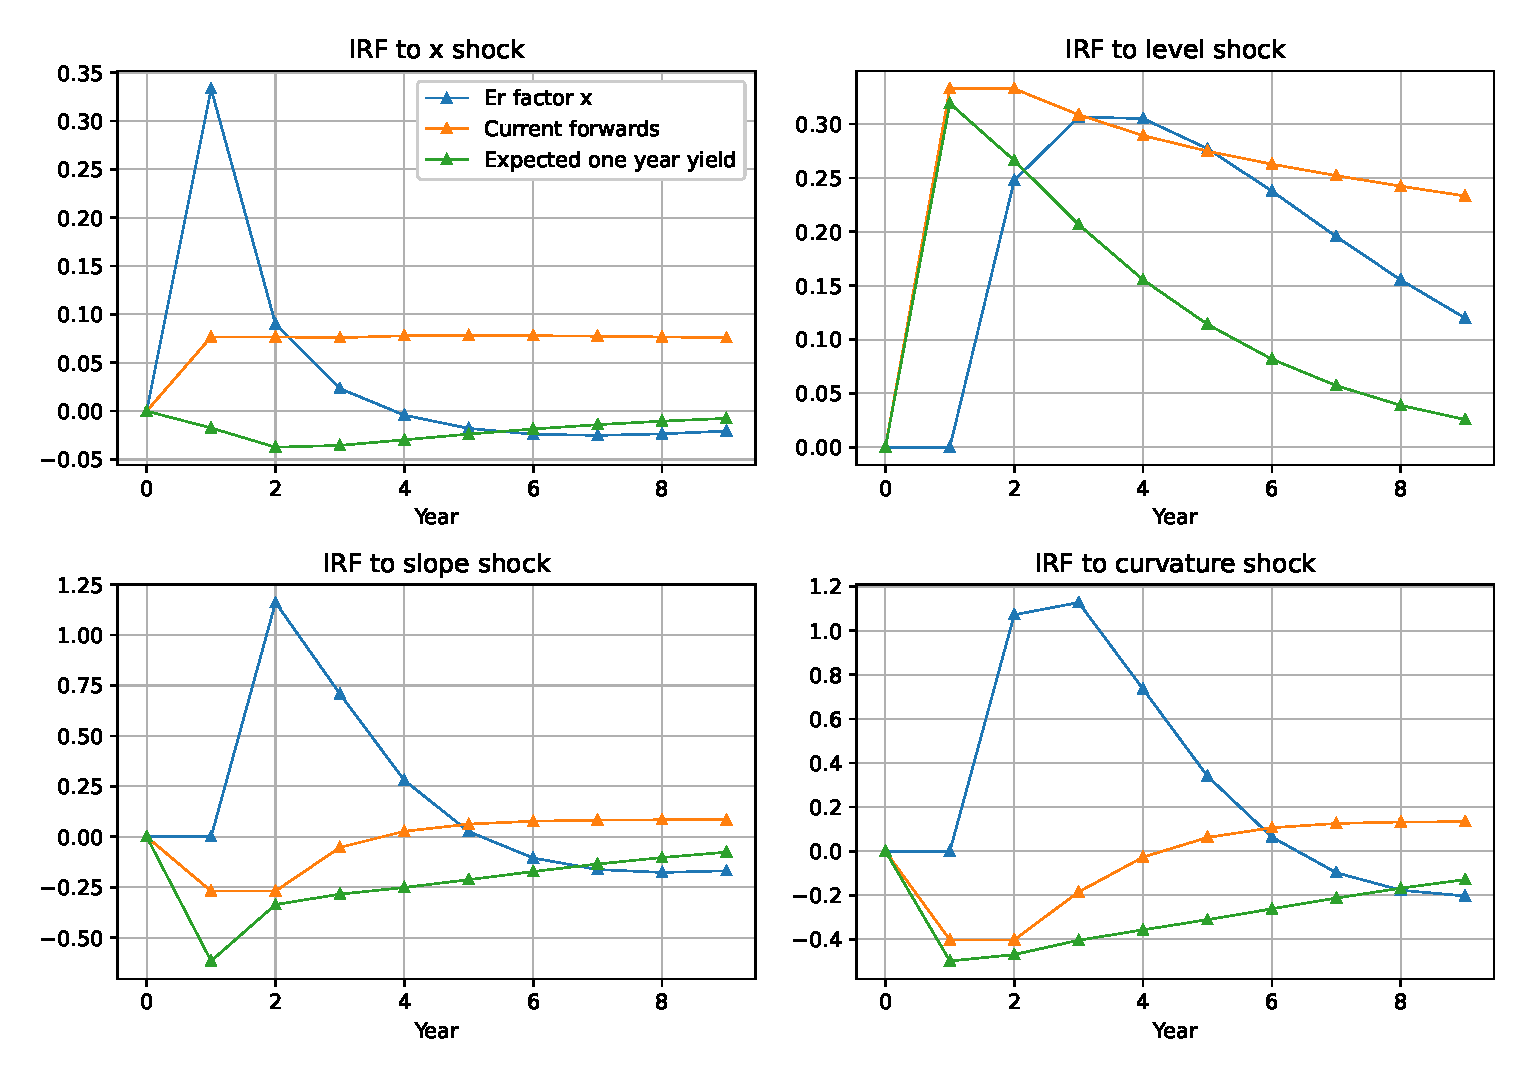
\includegraphics[scale=0.5]{fig/eps/Figure10.eps}
	\end{figure}


\end{document}